% !TeX program = xelatex
\documentclass[10pt, a4paper]{article}

\newif\ifpeerreview
\peerreviewfalse % Set \peerreviewtrue for anonymous Pintia peer-review submission

\usepackage{amsmath, amssymb, amsthm, mathtools}
\usepackage{geometry}
\usepackage{fancyhdr}
\usepackage{enumitem}
\usepackage{titlesec}
\usepackage{tocloft}
\usepackage[x11names]{xcolor}
\usepackage{graphicx}
\usepackage{float}
\usepackage{booktabs}
\usepackage{array}
\usepackage{multirow}
\usepackage{caption}
\usepackage{subcaption}
\usepackage{tikz}
\usepackage{microtype}
\usepackage{listings}
\usepackage[most]{tcolorbox}
\tcbuselibrary{skins, breakable}
\usepackage[backend=biber, citestyle=numeric-comp, bibstyle=numeric]{biblatex}
\usepackage{hyperref}
\usepackage{xurl}
\usepackage[capitalise, noabbrev]{cleveref}

\usetikzlibrary{arrows.meta, calc, positioning}

% --- Palette: Navy + Amber Gold + Sage ---
\definecolor{primary}{RGB}{28, 55, 90}
\definecolor{accent}{RGB}{176, 128, 52}
\definecolor{accentlight}{RGB}{232, 214, 178}
\definecolor{problembg}{RGB}{250, 248, 243}
\definecolor{problemframe}{RGB}{210, 220, 232}
\definecolor{textmuted}{RGB}{95, 105, 118}
\definecolor{coverbg}{RGB}{252, 249, 238}
\definecolor{progcolor}{RGB}{52, 105, 88}
\definecolor{alertred}{RGB}{168, 50, 50}

% --- Page Geometry & Header/Footer ---
\geometry{left=2.4cm, right=2.4cm, top=2.6cm, bottom=2.6cm}
\setlength{\headheight}{18pt}
\setlength{\parindent}{1.5em}
\setlength{\parskip}{0.38em}
\linespread{1.15}
\emergencystretch=2em
\setlist{nosep, leftmargin=1.8em}

\pagestyle{fancy}
\fancyhf{}
\fancyhead[L]{\small\color{primary}\textsf{ADS Project 5: Shopping with Coupons}}
\fancyhead[R]{\small\color{textmuted}\textsf{Fall--Winter 2026}}
\fancyfoot[C]{\small\color{textmuted}\thepage}
\renewcommand{\headrulewidth}{0.5pt}
\renewcommand{\headrule}{%
  {\color{accent!55}\hrule width\headwidth height 0.5pt}%
}

% --- Section & Subsection Headings ---
\titleformat{\section}
  {\color{primary}\centering\Large\bfseries}
  {\color{accent}Chapter~\thesection.}{0.6em}{}
  [\vspace{0.3em}{\color{accent!70}\titlerule[1.5pt]}]

\titleformat{name=\section,numberless}
  {\color{primary}\centering\Large\bfseries}
  {}{0pt}{}
  [\vspace{0.3em}{\color{accent!70}\titlerule[1.5pt]}]

\titleformat{\subsection}
  {\color{primary!88!black}\large\bfseries}
  {\color{accent}\thesubsection}{0.6em}{}
  [\vspace{0.15em}{\color{accent!45}\titlerule[0.8pt]}]

\titleformat{\subsubsection}
  {\color{primary!85!black}\normalsize\bfseries}
  {\color{accent}\thesubsubsection}{0.5em}{}

\titlespacing*{\section}{0pt}{0.6em}{1.0em}
\titlespacing*{\subsection}{0pt}{1.0em}{0.6em}
\titlespacing*{\subsubsection}{0pt}{0.8em}{0.4em}

% --- TOC Styling ---
\renewcommand{\cftsecfont}{\bfseries\color{primary}}
\renewcommand{\cftsecpagefont}{\bfseries\color{primary}}
\renewcommand{\cftsubsecfont}{\color{black!85}}
\renewcommand{\cftsubsubsecfont}{\small\color{textmuted}}
\setlength{\cftbeforesecskip}{0.55em}

% --- Styled Boxes ---
\newtcolorbox{theorembx}[1]{
    enhanced,
    breakable,
    colback=problembg,
    colframe=primary!30,
    boxrule=0.7pt,
    arc=3.5pt,
    borderline west={3.2pt}{0pt}{primary},
    left=12pt,
    right=12pt,
    top=7pt,
    bottom=8pt,
    before skip=7pt plus 2pt,
    after skip=8pt plus 2pt,
    title={\sffamily #1},
    fonttitle=\bfseries,
    coltitle=white,
    colbacktitle=primary,
    attach boxed title to top left={yshift=-2mm, xshift=8mm},
    boxed title style={
        arc=2.2pt,
        boxrule=0pt,
        top=1.8pt,
        bottom=1.8pt,
        left=6pt,
        right=6pt,
    },
}

\newtcolorbox{lemmabx}[1]{
    enhanced,
    breakable,
    colback=accentlight!22,
    colframe=accent!45,
    boxrule=0.65pt,
    arc=3.5pt,
    borderline west={3.0pt}{0pt}{accent!80},
    left=12pt,
    right=12pt,
    top=7pt,
    bottom=8pt,
    before skip=7pt plus 2pt,
    after skip=8pt plus 2pt,
    title={\sffamily #1},
    fonttitle=\bfseries,
    coltitle=primary,
    colbacktitle=accentlight!85,
    attach boxed title to top left={yshift=-2mm, xshift=8mm},
    boxed title style={
        arc=2.2pt,
        boxrule=0.5pt,
        colframe=accent!55,
        top=1.8pt,
        bottom=1.8pt,
        left=6pt,
        right=6pt,
    },
}

\newtcolorbox{insightbox}[1]{
    enhanced,
    breakable,
    colback=progcolor!5.5,
    colframe=progcolor!28,
    boxrule=0.7pt,
    arc=4pt,
    borderline west={3.5pt}{0pt}{progcolor},
    left=13pt,
    right=13pt,
    top=8pt,
    bottom=9pt,
    before skip=8pt plus 2pt,
    after skip=9pt plus 2pt,
    title={\sffamily #1},
    fonttitle=\bfseries,
    coltitle=white,
    colbacktitle=progcolor,
    attach boxed title to top left={yshift=-2mm, xshift=8mm},
    boxed title style={
        arc=2.5pt,
        boxrule=0pt,
        top=2pt,
        bottom=2pt,
        left=7pt,
        right=7pt,
    },
}

% --- Code Listings & Captions ---
\newcommand{\code}[1]{\texttt{\color{primary!90!black}#1}}
\newcommand{\kw}[1]{\textbf{\color{primary}#1}}
\newcommand{\id}[1]{\ensuremath{\mathrm{#1}}}
\captionsetup{labelfont={bf,color=primary}, skip=4pt}
\BeforeBeginEnvironment{tabular}{\small}

\lstset{
    language=C,
    basicstyle=\ttfamily\scriptsize,
    keywordstyle=\color{primary}\bfseries,
    commentstyle=\color{progcolor}\itshape,
    stringstyle=\color{accent},
    breaklines=true,
    numbers=left,
    numberstyle=\tiny\color{textmuted},
    frame=single,
    rulecolor=\color{problemframe},
    backgroundcolor=\color{problembg},
    captionpos=b,
    tabsize=4,
    columns=fullflexible,
    showstringspaces=false
}

\hypersetup{
    colorlinks=true,
    linkcolor=primary,
    citecolor=progcolor,
    urlcolor=accent,
    linktoc=all,
    pdfauthor={},
    pdftitle={Shopping with Coupons: Greedy Min-Heap Selection and Analysis}
}

\graphicspath{{../src/visualizations/}{../output/}{image/}{figure/}}
\addbibresource[location=local]{reference.bib}

\begin{document}

% ============================================================
%  PAGE 1: DEDICATED COVER + ABSTRACT PAGE
% ============================================================
\begin{titlepage}
\begin{tikzpicture}[remember picture, overlay]
    \fill[coverbg] (current page.south west) rectangle (current page.north east);
    \draw[accent!40, line width=0.7pt]
        ([xshift=1.5cm, yshift=-1.5cm]current page.north west) --
        ([xshift=1.5cm, yshift=1.5cm]current page.south west);
    \draw[accent!40, line width=0.7pt]
        ([xshift=-1.5cm, yshift=-1.5cm]current page.north east) --
        ([xshift=-1.5cm, yshift=1.5cm]current page.south east);
    \foreach \r in {2.0, 2.45, 2.9} {
        \draw[primary!14, line width=0.5pt]
            ([xshift=-1.35cm, yshift=1.35cm]current page.south east) circle (\r cm);
        \draw[primary!14, line width=0.5pt]
            ([xshift=1.35cm, yshift=-1.35cm]current page.north west) circle (\r cm);
    }
\end{tikzpicture}

\vspace*{0.7cm}
\begin{center}
    {\large\color{accent}\textsf{\textbf{Advanced Data Structures and Algorithm Analysis}}}\\[0.25cm]
    {\normalsize\color{textmuted}\textsf{Laboratory Project Report $\cdot$ Project 5}}\\[0.55cm]

    {\color{primary}\rule{0.58\textwidth}{1.4pt}}\\[0.5cm]
    {\fontsize{22}{29}\selectfont\bfseries\color{primary} Shopping with Coupons:}\\[0.2cm]
    {\fontsize{22}{29}\selectfont\bfseries\color{primary} Greedy Min-Heap Selection and Analysis}\\[0.45cm]
    {\color{accent}\rule{0.24\textwidth}{1.0pt}}\\[0.5cm]
    \ifpeerreview
        {\Large\bfseries\color{accent}\textsf{Group X}}\\[0.65cm]
        {\Large\bfseries\color{primary} Student A \hspace{2.8em} Student B}\\[0.35cm]
    \else
        {\Large\bfseries\color{accent}\textsf{Group 15}}\\[0.65cm]
        {\Large\bfseries\color{primary} Yixiang Chen \hspace{2.8em} Runhui Lin}\\[0.35cm]
    \fi
    {\normalsize\color{textmuted}
        Zhejiang University \\[0.15cm]
        Date: 2026-11-23
    }
\end{center}

\vspace{0.55cm}
\begin{center}
    {\large\bfseries\color{primary} Abstract}
\end{center}
\vspace{-0.25em}
\begin{quote}
\small\noindent
In the \textbf{Shopping with Coupons} problem, a shopper with budget $D \le 10^6$ faces $N \le 10^5$ item types of prices $P_1, \ldots, P_N$ and $N$ coupon types of discounts $C_1, \ldots, C_N$ satisfying $\max_j C_j < \min_i P_i$. Each item--coupon pair $(i, j)$ may be redeemed at most once at net cost $P_i - C_j$, at most one coupon applies per purchased unit, and full-price purchases are unlimited; the goal is to maximize total items bought and, secondarily, maximize remaining money. Materializing all $N^2$ discounted pairs requires $\Theta(N^2)$ memory and $\Omega(N^2)$ time, reaching $\mathbf{10^{10}}$ pairs at $N = 10^5$. Exploiting monotonicity of sorted discounts $C_{(1)} \ge \cdots \ge C_{(N)}$, we implement an $N$-way frontier greedy solver in C11 combining median-of-three \textbf{three-way QuickSort}, a capacity-$N$ \textbf{binary min-heap}, and an \textbf{$O(1)$ bulk-purchase cutoff} at the minimum original price $B = \min_i P_i$. Cross-checked against an independent $O(N \log N + N \log D)$ binary-search and prefix-sum oracle across \textbf{$158$ test cases} spanning $6$ distributions and $13$ sizes up to $N = 10^5$ plus $2$ boundary checks, our solver achieves \textbf{$100\%$ exact agreement} on item count, remaining money, and coupon-purchase count $K$. At $N = 10^5$, mean runtime spans \textbf{$\mathbf{4.47\text{--}11.03\,\text{ms}}$} across all six profiles---even when $K = 10^6$---confirming the parameterized average-case bound $O((N + K)\log N)$ in $\Theta(N)$ auxiliary space.

\vspace{0.5em}\noindent
{\color{primary}\textbf{Keywords:}} greedy algorithm; binary min-heap; three-way quicksort; time and space complexity.
\end{quote}

\vfill
\begin{center}
    {\color{accent!80}\rule{0.14\textwidth}{0.8pt}}\\[0.25cm]
    {\normalsize\bfseries\color{primary} Fall--Winter 2026}
\end{center}
\end{titlepage}

% ============================================================
%  PAGE 2: DEDICATED TABLE OF CONTENTS PAGE
% ============================================================
\pagenumbering{roman}
\thispagestyle{plain}
\vspace*{0.3cm}
\tableofcontents
\clearpage

% ============================================================
%  CHAPTER 1: INTRODUCTION
% ============================================================
\pagenumbering{arabic}
\section{Introduction}

\subsection{Problem Description}
Let $N \in \{1, \ldots, 10^5\}$ denote both the number of item types and the number of coupon types, and let $D \in \{1, \ldots, 10^6\}$ denote the budget in dollars. Item type $i \in \{1, \ldots, N\}$ has original price $P_i \in [1, 10^9]$, and coupon type $j \in \{1, \ldots, N\}$ gives discount $C_j \in [1, 10^9]$ with $\max_{1 \le j \le N} C_j < \min_{1 \le i \le N} P_i$.

Each purchased unit uses at most one coupon, full-price purchases are unlimited, and each specific pair $(i, j) \in \{1, \ldots, N\}^2$ can be redeemed \emph{at most once}. Let $x_{i,j} \in \{0, 1\}$ indicate whether coupon $j$ is applied to one unit of item $i$ at net cost $P_i - C_j \ge 1$, and let $y_i \in \mathbb{Z}_{\ge 0}$ count full-price units of item $i$. A feasible plan $(x, y)$ with expenditure $E(x, y) \le D$ yields unit count $Q(x, y)$:
\begin{equation}
  Q(x, y) \;=\; \sum_{i=1}^{N} \sum_{j=1}^{N} x_{i,j} + \sum_{i=1}^{N} y_i,
  \qquad
  E(x, y) \;=\; \sum_{i=1}^{N} \sum_{j=1}^{N} (P_i - C_j)\, x_{i,j} + \sum_{i=1}^{N} P_i\, y_i.
  \label{eq:quantity-cost}
\end{equation}
The \textbf{Shopping with Coupons} problem first maximizes total items bought and then maximizes remaining money:
\begin{equation}
  Q^* \;=\; \max_{\substack{x \in \{0,1\}^{N \times N},\; y \in \mathbb{Z}_{\ge 0}^N \\ E(x, y) \le D}} Q(x, y),
  \qquad
  R^* \;=\; D \;-\; \min_{\substack{x \in \{0,1\}^{N \times N},\; y \in \mathbb{Z}_{\ge 0}^N \\ E(x, y) \le D,\; Q(x, y) = Q^*}} E(x, y).
  \label{eq:lex-opt}
\end{equation}

Since every unit contributes $+1$ to $Q(x, y)$, greedy selection in non-decreasing order of marginal cost simultaneously achieves $Q^*$ and $R^*$~\cite{ads_slides2026, cormen2022}. Scaling to $N = 10^5$ and $D = 10^6$ hinges on four design choices:
\begin{itemize}
  \item \textbf{\color{primary}Avoiding $\Theta(N^2)$ Pair Enumeration:} Materializing all $N^2$ discounted costs $P_i - C_j$ creates $10^{10}$ entries, or roughly $40\,\text{GiB}$ at $N = 10^5$, making explicit sorting infeasible in both time and memory.
  \item \textbf{\color{primary}Per-Item Sorted Frontier via Binary Min-Heap:} Sorting discounts once as $C_{(1)} \ge \cdots \ge C_{(N)}$ orders each item's discounted prices as $P_i - C_{(1)} \le \cdots \le P_i - C_{(N)}$. Keeping only the $N$ current cheapest per-item entries in a binary min-heap~\cite{ads_slides2026, weiss1996} streams minimum pairs in $\Theta(N)$ space.
  \item \textbf{\color{primary}Original-Price Bulk Cutoff at $B = \min_i P_i$:} Let $B = \min_{1 \le i \le N} P_i$ be the cheapest full price. Any option costing at least $B$ is matched or beaten by unlimited full-price units at $B$; stopping heap pops once $\min \mathcal{H} \ge B$ collapses all remaining $\lfloor D_{\text{rem}} / B \rfloor$ units into one $O(1)$ division.
  \item \textbf{\color{primary}Three-Way QuickSort and Threshold Oracle:} Coupons are ordered by median-of-three three-way QuickSort with a selection-sort cutoff at $16$~\cite{weiss1996, cormen2022}, and every run is cross-checked against an independent $O(N \log N + N \log D)$ binary-search and prefix-sum oracle.
\end{itemize}

\subsection{Purpose of This Report}
This report designs, verifies, and analyzes our C11 solver for \textbf{Shopping with Coupons}:
\begin{enumerate}[label=\textbf{\color{primary}\arabic*.}]
  \item \textbf{Specify Data Structures and Algorithms:} Document the custom min-heap, three-way QuickSort, greedy frontier solver with $O(1)$ bulk cutoff, and threshold verification oracle in Chapter~2.
  \item \textbf{Verify and Benchmark Six Input Regimes:} Evaluate $158$ deterministic cases from \code{generate.c} across $N \in [16, 10^5]$ and six synthetic distributions---\code{random}, \code{duplicates}, \code{near\_limit}, \code{unaffordable}, \code{many\_purchases}, and \code{ordered}---in Chapter~3.
  \item \textbf{Prove Optimality and Parameterized Complexity:} Prove greedy optimality for $(Q^*, R^*)$, derive the output-sensitive $O((N + K)\log N)$ average-case bound in coupon-purchase count $K$, and explain empirical regressions and architectural effects in Chapter~4.
\end{enumerate}

\clearpage

% ============================================================
%  CHAPTER 2: DATA STRUCTURE AND ALGORITHM SPECIFICATION
% ============================================================
\section{Data Structure and Algorithm Specification}

\subsection{Overview of Solver and Benchmark Data Structures}
\Cref{tab:structures} summarizes the C11 structures across \code{shopping\_with\_cunpons.h}, \code{binary\_min\_heap.h}, \code{bench.h}, and \code{testbench.c}. Instead of materializing all $N^2$ discounted pairs, our solver maintains an $N$-element item-cursor array alongside a capacity-$N$ parallel-array binary min-heap, keeping peak auxiliary memory strictly linear in $N$.

\begin{table}[H]
\centering
\caption{Core solver and verification data structures in \code{src/}.}
\label{tab:structures}
\begin{tabular}{@{}l>{\raggedright\arraybackslash}p{0.34\linewidth}>{\raggedright\arraybackslash}p{0.42\linewidth}@{}}
\toprule
\textbf{\color{primary}Structure} & \textbf{\color{primary}C Fields / Layout} & \textbf{\color{primary}Structural Invariant \& Role} \\
\midrule
\code{Item} & \code{int price}, \code{int couponIndex} & Stores item $i$'s base price $P_i$ and cursor $\id{couponIndex}_i \in \{0, \ldots, N\}$ to its next unredeemed coupon in sorted \code{coupons[]}. \\
\code{BinaryMinHeap} & \code{int64\_t *data}, \code{int *vertices}, \code{int size}, \code{int capacity} & 0-indexed parallel-array min-heap of size $\le N$; slot $t$ pairs discounted cost $\code{data}[t] = P_v - C_{(\id{idx}_v)}$ with item ID $v = \code{vertices}[t]$, obeying $\code{data}[\lfloor(t-1)/2\rfloor] \le \code{data}[t]$. \\
\code{Result} & \code{int count}, \code{int money} & Output record $(Q^*, R^*)$ returned by both solver and oracle; \code{\{-1, -1\}} signals allocation failure. \\
\code{Stats} & \code{int64\_t count}, \code{int64\_t cost} & 64-bit cumulative unit count and dollar cost of all options with marginal price $\le t$ in \code{testbench.c}. \\
\bottomrule
\end{tabular}
\end{table}

\subsection{Three-Way Partitioned QuickSort for Coupon Ordering}
To stream discounted prices for each item $i$ in non-decreasing order without sorting $N$ rows separately, \code{solveShoppingCounted} first sorts \code{coupons[0..N-1]} in \emph{non-increasing} order $C_{(0)} \ge C_{(1)} \ge \cdots \ge C_{(N-1)}$ via \code{quickSort} in \code{quick\_sort.h}. For every fixed item $i$, the row sequence $P_i - C_{(0)} \le P_i - C_{(1)} \le \cdots \le P_i - C_{(N-1)}$ is then automatically non-decreasing.

Standard two-way QuickSort degrades to $\Theta(N^2)$ when coupon discounts contain heavy duplicates---such as \code{many\_purchases} with $C_j \equiv 1$ or \code{duplicates} with $C_j \in [95, 99]$---or already ordered inputs. Our implementation in \code{quick\_sort.h} combines three standard safeguards~\cite{ads_slides2026, weiss1996}:
\begin{itemize}
  \item \textbf{\color{primary}Small-Subarray Selection Cutoff at $\code{THRESHOLD} = 16$:} Subarrays with $\id{right} - \id{left} + 1 \le 16$ switch to in-place descending \code{selectionSort}, avoiding recursion overhead on tiny leaves.
  \item \textbf{\color{primary}Median-of-Three Pivot:} Three conditional swaps order $\code{a[left]} \ge \code{a[mid]} \ge \code{a[right]}$ for $\id{mid} = \id{left} + \lfloor(\id{right} - \id{left})/2\rfloor$, selecting $\id{pivot} = \code{a[mid]}$ as a central splitter.
  \item \textbf{\color{primary}Three-Way Partitioning and Tail-Call Elimination:} Cursors $(\id{lt}, i, \id{gt})$ partition $\code{a[left..right]}$ in one pass into $> \id{pivot}$, $= \id{pivot}$, and $< \id{pivot}$ zones; all keys equal to $\id{pivot}$ settle permanently into $\code{a[lt..gt]}$. Recursing only on the smaller outer slice while iterating on the larger slice via the enclosing \kw{while} loop caps call-stack depth at $\lfloor \log_2 N \rfloor$.
\end{itemize}

\begin{table}[H]
\centering
\begin{tabular}{@{}p{2.15cm}p{0.77\textwidth}@{}}
\toprule
\multicolumn{2}{@{}l}{\textbf{\color{primary}Algorithm 1:} Descending Three-Way QuickSort $\id{quickSort}(a, \id{left}, \id{right})$ in \code{quick\_sort.h}} \\
\midrule
\textbf{QuickSort:} &
1. \kw{while} $\id{left} < \id{right}$ \kw{do} \\
& 2. \quad \kw{if} $\id{right} - \id{left} + 1 \le 16$ \kw{then} $\id{selectionSort}(a, \id{left}, \id{right})$ descending; \kw{return}. \\
& 3. \quad Let $\id{mid} \gets \id{left} + \lfloor(\id{right} - \id{left})/2\rfloor$; sort $(a[\id{left}], a[\id{mid}], a[\id{right}])$ descending; set $p \gets a[\id{mid}]$. \\
& 4. \quad Initialize $\id{lt} \gets \id{left}$, $i \gets \id{left}$, $\id{gt} \gets \id{right}$. \\
& 5. \quad \kw{while} $i \le \id{gt}$ \kw{do} \\
& 6. \quad\quad \kw{if} $a[i] > p$ \kw{then} $\id{swap}(a[\id{lt}\text{++}], a[i\text{++}])$ \kw{else if} $a[i] < p$ \kw{then} $\id{swap}(a[i], a[\id{gt}\text{--}])$ \kw{else} $i\text{++}$. \\
& 7. \quad \kw{if} $\id{lt} - \id{left} < \id{right} - \id{gt}$ \kw{then} $\id{quickSort}(a, \id{left}, \id{lt} - 1)$; $\id{left} \gets \id{gt} + 1$. \\
& 8. \quad \kw{else} $\id{quickSort}(a, \id{gt} + 1, \id{right})$; $\id{right} \gets \id{lt} - 1$. \\
\bottomrule
\end{tabular}
\end{table}

\subsection{Binary Min-Heap and Greedy Frontier Solver}
Once discounts satisfy $C_{(0)} \ge \cdots \ge C_{(N-1)}$, the $N^2$ discounted costs form an implicit $N \times N$ row-sorted matrix $M_{i,j} = P_i - C_{(j)}$ for $0 \le i, j < N$. In \code{binary\_min\_heap.h}, \code{BinaryMinHeap} stores at most one active frontier entry per row using two contiguous arrays: \code{int64\_t data[]} for marginal prices and \code{int vertices[]} for row indices $i$. Storing keys as 64-bit signed integers allows \code{getMin} to return \code{INT64\_MAX} cleanly on an empty heap without colliding with valid prices up to $10^9$. Standard 0-based \code{siftup}, comparing slot $t$ against parent $\lfloor(t-1)/2\rfloor$, and \code{siftdown}, comparing against children $2t+1$ and $2t+2$ under strict inequality \code{<}, maintain the min-heap invariant in $O(\log N)$ swaps.

In \code{shopping\_with\_cunpons.h}, \code{solveShoppingCounted} scans $i = 0, \ldots, N-1$ to record the minimum full price $B = \min_{0 \le i < N} P_i$ and inserts every row head $(P_i - C_{(0)}, i)$ into \code{heap}. Each iteration of the greedy loop maintains the \textbf{Frontier Invariant}: for every item $i$, coupons $0, \ldots, \id{idx}_i - 1$ have been redeemed, and if $\id{idx}_i < N$, entry $(P_i - C_{(\id{idx}_i)}, i)$ is in \code{heap}; hence \code{getMin(heap)} equals the minimum cost among all unredeemed coupon pairs. Before extracting the root, the solver tests the \textbf{bulk-cutoff condition} $\id{isEmpty}(\mathcal{H}) \lor \id{getMin}(\mathcal{H}) \ge B$:
\begin{itemize}
  \item \textbf{\color{primary}$O(1)$ Bulk Full-Price Termination:} If no unredeemed coupon pair costs strictly less than $B$, buying the cheapest item at full price $B$ dominates all remaining couponed and uncouponed options. The solver adds $\lfloor D_{\text{rem}} / B \rfloor$ to \code{maxItems}, updates $D_{\text{rem}} \gets D_{\text{rem}} \bmod B$, and exits the loop immediately.
  \item \textbf{\color{primary}$O(\log N)$ Heap Frontier Advance:} Otherwise $\id{minPrice} = \id{getMin}(\mathcal{H}) < B$. If $D_{\text{rem}} < \id{minPrice}$, no further unit is affordable and the loop terminates; else $D_{\text{rem}}$ decreases by $\id{minPrice}$, both \code{maxItems} and coupon-purchase counter $K$ increment, root $(P_v - C_{(\id{idx}_v)}, v)$ is popped, $\id{idx}_v$ increments, and if $\id{idx}_v < N$ the successor $(P_v - C_{(\id{idx}_v)}, v)$ is pushed into $\mathcal{H}$.
\end{itemize}
Algorithm~2 formalizes this procedure, and \Cref{fig:frontier_trace} illustrates the implicit matrix frontier and cutoff gate on the four-item sample instance at $D = 30$.

\begin{table}[H]
\centering
\begin{tabular}{@{}p{2.15cm}p{0.77\textwidth}@{}}
\toprule
\multicolumn{2}{@{}l}{\textbf{\color{primary}Algorithm 2:} Greedy Frontier Solver $\id{solveShoppingCounted}(N, D, P, C, \&K)$ in \code{shopping\_with\_cunpons.h}} \\
\midrule
\textbf{Initialize:} &
1. Sort $C[0..N-1]$ in non-increasing order via $\id{quickSort}(C, 0, N-1)$. \\
& 2. Set $D_{\text{rem}} \gets D$, $Q \gets 0$, $K \gets 0$, $B \gets P[0]$, and create capacity-$N$ min-heap $\mathcal{H}$. \\
& 3. \kw{for} $i = 0$ \kw{to} $N - 1$ \kw{do}: $\id{idx}[i] \gets 0$; $B \gets \min(B, P[i])$; $\id{insert}(\mathcal{H}, P[i] - C[0], i)$. \\[0.25em]
\textbf{Greedy:} &
4. \kw{while} $D_{\text{rem}} > 0$ \kw{do} \\
& 5. \quad \kw{if} $\id{isEmpty}(\mathcal{H})$ \kw{or} $\id{getMin}(\mathcal{H}) \ge B$ \kw{then} \\
& 6. \quad\quad $Q \gets Q + \lfloor D_{\text{rem}} / B \rfloor$; $\;D_{\text{rem}} \gets D_{\text{rem}} \bmod B$; \;\kw{break}. \\
& 7. \quad Let $m \gets \id{getMin}(\mathcal{H})$; \;\kw{if} $D_{\text{rem}} < m$ \kw{then break}. \\
& 8. \quad $D_{\text{rem}} \gets D_{\text{rem}} - m$; $\;Q \gets Q + 1$; $\;K \gets K + 1$; $\;\id{extractMin}(\mathcal{H}, \&m, \&v)$. \\
& 9. \quad $\id{idx}[v] \gets \id{idx}[v] + 1$; \;\kw{if} $\id{idx}[v] < N$ \kw{then} $\id{insert}(\mathcal{H}, P[v] - C[\id{idx}[v]], v)$. \\
& 10. Free $\mathcal{H}$ and $\id{idx}[]$; \;\kw{return} $(Q, D_{\text{rem}})$ and coupon-purchase count $K$. \\
\bottomrule
\end{tabular}
\end{table}

\begin{figure}[H]
\centering
\begin{tikzpicture}[
  x=1.0cm, y=0.82cm,
  font=\scriptsize,
  bought/.style={draw=progcolor, thick, rounded corners=2pt, fill=progcolor!12, text=primary, minimum width=10.8mm, minimum height=5.8mm, align=center, font=\scriptsize\bfseries},
  front/.style={draw=accent, very thick, rounded corners=2pt, fill=accentlight!55, text=primary, minimum width=10.8mm, minimum height=5.8mm, align=center, font=\scriptsize\bfseries},
  unvis/.style={draw=problemframe!95!black, rounded corners=2pt, fill=white, text=primary!85, minimum width=10.8mm, minimum height=5.8mm, align=center},
  domcell/.style={draw=alertred!65, dashed, rounded corners=2pt, fill=alertred!7, text=alertred!85!black, minimum width=10.8mm, minimum height=5.8mm, align=center},
  hnode/.style={draw=primary, thick, circle, fill=problembg, text=primary, inner sep=1.5pt, minimum size=8.4mm, align=center, font=\tiny\bfseries}
]
  % Title Left
  \node[font=\scriptsize\bfseries\color{primary}] at (2.85, 4.15) {Implicit Sorted-Row Matrix $M_{i,j} = P_i - C_{(j)}$ at $B = 10$};

  % Column labels
  \node[font=\tiny\bfseries\color{textmuted}] at (1.20, 3.45) {$C_{(0)}\!=\!9$};
  \node[font=\tiny\bfseries\color{textmuted}] at (2.45, 3.45) {$C_{(1)}\!=\!8$};
  \node[font=\tiny\bfseries\color{textmuted}] at (3.70, 3.45) {$C_{(2)}\!=\!7$};
  \node[font=\tiny\bfseries\color{textmuted}] at (4.95, 3.45) {$C_{(3)}\!=\!6$};

  % Row labels
  \node[anchor=east, font=\scriptsize\bfseries\color{primary}] at (0.52, 2.70) {$i\!=\!0,\;P\!=\!12$};
  \node[anchor=east, font=\scriptsize\bfseries\color{primary}] at (0.52, 1.80) {$i\!=\!1,\;P\!=\!20$};
  \node[anchor=east, font=\scriptsize\bfseries\color{primary}] at (0.52, 0.90) {$i\!=\!2,\;P\!=\!15$};
  \node[anchor=east, font=\scriptsize\bfseries\color{primary}] at (0.52, 0.00) {$i\!=\!3,\;P\!=\!10$};

  % Row 0: P=12 -> 3, 4, 5, 6
  \node[bought] (m00) at (1.20, 2.70) {$3_{\,\#3}$};
  \node[bought] (m01) at (2.45, 2.70) {$4_{\,\#5}$};
  \node[bought] (m02) at (3.70, 2.70) {$5_{\,\#7}$};
  \node[front]  (m03) at (4.95, 2.70) {$6$};

  % Row 1: P=20 -> 11, 12, 13, 14
  \node[domcell] (m10) at (1.20, 1.80) {$11$};
  \node[domcell] (m11) at (2.45, 1.80) {$12$};
  \node[domcell] (m12) at (3.70, 1.80) {$13$};
  \node[domcell] (m13) at (4.95, 1.80) {$14$};

  % Row 2: P=15 -> 6, 7, 8, 9
  \node[bought] (m20) at (1.20, 0.90) {$6_{\,\#8}$};
  \node[front]  (m21) at (2.45, 0.90) {$7$};
  \node[unvis]  (m22) at (3.70, 0.90) {$8$};
  \node[unvis]  (m23) at (4.95, 0.90) {$9$};

  % Row 3: P=10 -> 1, 2, 3, 4
  \node[bought] (m30) at (1.20, 0.00) {$1_{\,\#1}$};
  \node[bought] (m31) at (2.45, 0.00) {$2_{\,\#2}$};
  \node[bought] (m32) at (3.70, 0.00) {$3_{\,\#4}$};
  \node[bought] (m33) at (4.95, 0.00) {$4_{\,\#6}$};

  % Highlight frontier border on m10 too
  \draw[accent, very thick, rounded corners=2pt] (m10.south west) rectangle (m10.north east);

  % Right Panel: Initial vs Final Heap + Bulk Cutoff Gate
  \node[font=\scriptsize\bfseries\color{primary}] at (9.65, 4.15) {Min-Heap $\mathcal{H}$ of Size $\le N$ \& Cutoff Gate};

  % Initial Heap subbox
  \node[font=\tiny\bfseries\color{textmuted}] at (7.85, 3.45) {Init: $D_{\text{rem}}\!=\!30$};
  \node[hnode, fill=progcolor!12, draw=progcolor] (h0) at (7.85, 2.65) {$1$\\[-2pt]$i\!=\!3$};
  \node[hnode] (h1) at (7.10, 1.50) {$3$\\[-2pt]$i\!=\!0$};
  \node[hnode] (h2) at (8.60, 1.50) {$6$\\[-2pt]$i\!=\!2$};
  \node[hnode, draw=alertred!75] (h3) at (6.65, 0.35) {$11$\\[-2pt]$i\!=\!1$};
  \draw[thick, primary!70] (h0) -- (h1);
  \draw[thick, primary!70] (h0) -- (h2);
  \draw[thick, primary!70] (h1) -- (h3);

  % Arrow to K=8 Heap
  \draw[-{Stealth[length=1.8mm]}, very thick, accent] (9.15, 2.05) -- node[above, font=\tiny\bfseries\color{primary}]{$K\!=\!8$ pops} node[below, font=\tiny\color{textmuted}]{spent $\$28$} (10.25, 2.05);

  % Final Heap after K=8 pops
  \node[font=\tiny\bfseries\color{textmuted}] at (11.35, 3.45) {Stop: $D_{\text{rem}}\!=\!2$};
  \node[hnode, fill=accentlight!55, draw=accent] (f0) at (11.35, 2.65) {$6$\\[-2pt]$i\!=\!0$};
  \node[hnode, fill=accentlight!55, draw=accent] (f1) at (10.65, 1.50) {$7$\\[-2pt]$i\!=\!2$};
  \node[hnode, draw=alertred!75] (f2) at (12.05, 1.50) {$11$\\[-2pt]$i\!=\!1$};
  \draw[thick, primary!70] (f0) -- (f1);
  \draw[thick, primary!70] (f0) -- (f2);

  % Decision note box at bottom right
  \node[draw=primary!35, fill=problembg, rounded corners=2.5pt, inner sep=3.2pt, text width=5.35cm, align=left, font=\tiny\color{primary}] at (9.65, -0.35) {%
    \textbf{Stop / Cutoff Rules:} Row $i\!=\!3$ exhausts all $4$ coupons; at $K\!=\!8$, $\min \mathcal{H}\!=\!6 > D_{\text{rem}}\!=\!2 \Rightarrow$ return $(Q^*\!=\!8, R^*\!=\!2)$. If $\min \mathcal{H} \ge B\!=\!10$ first, buy $\lfloor D_{\text{rem}}/B \rfloor$ units in $O(1)$.};

  % Legend bar across bottom
  \node[bought, minimum width=8.2mm, minimum height=4.4mm] at (-0.65, -1.25) {$m_{\#k}$};
  \node[anchor=west, font=\tiny\color{primary}] at (-0.15, -1.25) {Popped at step $k$};
  \node[front, minimum width=7.5mm, minimum height=4.4mm] at (2.45, -1.25) {$m$};
  \node[anchor=west, font=\tiny\color{primary}] at (2.92, -1.25) {Active heap frontier};
  \node[unvis, minimum width=7.5mm, minimum height=4.4mm] at (5.80, -1.25) {$m$};
  \node[anchor=west, font=\tiny\color{textmuted}] at (6.27, -1.25) {Unvisited $< B$};
  \node[domcell, minimum width=7.5mm, minimum height=4.4mm] at (8.70, -1.25) {$m$};
  \node[anchor=west, font=\tiny\color{alertred!85!black}] at (9.17, -1.25) {Dominated, $\ge B\!=\!10$};
\end{tikzpicture}
\caption{\footnotesize Implicit sorted-row matrix $M_{i,j} = P_i - C_{(j)}$ and min-heap frontier on the four-item sample instance.}
\label{fig:frontier_trace}
\end{figure}

\subsection{Independent Threshold-Search Verification Oracle}
To verify functional correctness without sharing any priority-queue or greedy simulation code, \code{testbench.c} implements an independent reference routine \code{oracle} with helper \code{statsAt} based on binary search over marginal unit cost $t \in [0, D]$.

After sorting local copies $p[0] \le \cdots \le p[N-1]$ and $c[0] \le \cdots \le c[N-1]$ via C's \code{qsort} and precomputing 64-bit prefix sums $\id{prefix}[m] = \sum_{r=0}^{m-1} c[r]$, \code{statsAt(t)} counts all pairs satisfying $p[i] - c[j] \le t$, equivalently $c[j] \ge p[i] - t$, in $O(N)$ time: as $i$ increases from $0$ to $N-1$, threshold $p[i] - t$ is non-decreasing, so pointer $j$ advances monotonically from $0$ to $N$, contributing $k_i = N - j$ pairs of aggregate cost $k_i p[i] - (\id{prefix}[N] - \id{prefix}[j])$. Whenever $t \ge p[0]$, up to $\lfloor D / p[0] \rfloor$ full-price units of item $p[0]$ are also included. Binary search over $t \in [0, D]$ finds the largest threshold $t^*$ with $\id{cost}(t^*) \le D$ in $\lceil \log_2(D + 1) \rceil \le 20$ probes, purchases as many boundary units at price $t^* + 1$ as $D - \id{cost}(t^*)$ permits, and independently checks $K^* = \min\bigl(Q^*, \id{count}(p[0] - 1)\bigr)$.

\begin{table}[H]
\centering
\begin{tabular}{@{}p{2.15cm}p{0.77\textwidth}@{}}
\toprule
\multicolumn{2}{@{}l}{\textbf{\color{primary}Algorithm 3:} Binary-Search \& Two-Pointer Oracle $\id{oracle}(N, D, P, C, \&K^*)$ in \code{testbench.c}} \\
\midrule
\textbf{statsAt($t$):} &
1. Set $\id{cnt} \gets 0$, $\id{cost} \gets 0$, $j \gets 0$. \\
& 2. \kw{for} $i = 0$ \kw{to} $N - 1$ \kw{do}: \kw{while} $j < N$ \kw{and} $c[j] < p[i] - t$ \kw{do} $j\text{++}$; add $k_i = N - j$ to $\id{cnt}$ and $k_i p[i] - (\id{prefix}[N] - \id{prefix}[j])$ to $\id{cost}$. \\
& 3. \kw{if} $t \ge p[0]$ \kw{then} add $b = \lfloor D / p[0] \rfloor$ to $\id{cnt}$ and $b \cdot p[0]$ to $\id{cost}$; \;\kw{return} $(\id{cnt}, \id{cost})$. \\[0.25em]
\textbf{Oracle:} &
4. Copy and sort $p[0..N-1]$ and $c[0..N-1]$ ascending; build $\id{prefix}[0..N]$ of $c[]$. \\
& 5. Binary search $\id{low} \gets 0, \id{high} \gets D$ for largest $t^* = \id{low}$ with $\id{statsAt}(t^*).\id{cost} \le D$. \\
& 6. Let $(\id{cnt}_0, \id{cost}_0) \gets \id{statsAt}(t^*)$; if $t^* < D$, let $\id{extra} \gets \min\bigl(\lfloor(D - \id{cost}_0)/(t^* + 1)\rfloor,\; \id{statsAt}(t^*+1).\id{cnt} - \id{cnt}_0\bigr)$, else $0$. \\
& 7. Set $Q^* \gets \id{cnt}_0 + \id{extra}$, $R^* \gets D - \id{cost}_0 - \id{extra}\cdot(t^* + 1)$, $K^* \gets \min(Q^*, \id{statsAt}(p[0]-1).\id{cnt})$; \;\kw{return} $(Q^*, R^*)$. \\
\bottomrule
\end{tabular}
\end{table}

\clearpage

% ============================================================
%  CHAPTER 3: TESTING RESULTS
% ============================================================
\section{Testing Results}

\subsection{Dataset Generator and Benchmark Protocol}
All benchmark inputs are deterministically synthesized by \code{src/generate.c} using a 32-bit xorshift generator seeded with $\id{seed} = 20261123 + 100\,\id{slot}(N) + 10\,\id{mode} + \id{trial}$ and rejection-sampled uniform integers via \code{between} to avoid modulo bias. Across $13$ problem sizes
\[
  N \;\in\; \{16, 32, 64, 100, 256, 512, 1000, 2000, 5000, 10000, 20000, 50000, 100000\},
\]
six structural distributions listed in \Cref{tab:profiles} are instantiated with two seeds each at fixed budget $D = 1{,}000{,}000$, yielding $13 \times 6 \times 2 = 156$ scaling instances plus $2$ known-answer unit cases \code{sample.in} and \code{original\_price.in}, for $158$ cases indexed in \code{data/manifest.csv}.

\begin{table}[H]
\centering
\caption{Synthetic benchmark profiles generated by \code{src/generate.c} at $D = 10^6$.}
\label{tab:profiles}
\renewcommand{\arraystretch}{1.0}
\setlength{\tabcolsep}{4.2pt}
\footnotesize
\begin{tabular}{@{}lrr>{\raggedright\arraybackslash}p{0.44\linewidth}@{}}
\toprule
\textbf{\color{primary}Profile} & \textbf{\color{primary}Price Range $P_i$} & \textbf{\color{primary}Coupon Range $C_j$} & \textbf{\color{primary}Target Stress Regime} \\
\midrule
\code{random}         & $[1{,}000,\; 2{,}000]$         & $[1,\; 999]$                   & General uncorrelated costs; moderate $K$ up to $2.2 \times 10^5$. \\
\code{duplicates}     & $[100,\; 105]$                 & $[95,\; 99]$                   & Narrow $5$-value bands; massive key ties and $K$ up to $10^6$. \\
\code{near\_limit}    & $[10^9 - 100,\; 10^9]$         & $[10^9 - 200,\; 10^9 - 101]$   & Extreme $10^9$ magnitudes with small net gaps $P_i - C_j \in [1, 200]$. \\
\code{unaffordable}   & $[5 \times 10^8,\; 10^9]$      & $[1,\; 10^6]$                  & Net cost $\ge 4.99 \times 10^8 > D$; forces $K = 0$ to isolate sort and init. \\
\code{many\_purchases}& $[2,\; 3]$                     & $\{1\}$                        & Identical coupons, $Q^*$ up to $10^6$, and heavy $O(1)$ bulk cutoff at small $N$. \\
\code{ordered}        & $100{,}001 + i$                & $i + 1$ or $N - i$             & Strictly ascending $P_i$ with ascending or descending $C_j$ for pivot stress. \\
\bottomrule
\end{tabular}
\end{table}

In \code{src/testbench.c}, compiled with \texttt{gcc -O2 -std=c11}, each instance is validated for domain bounds and $\max_j C_j < \min_i P_i$, solved once by the independent binary-search \code{oracle}, warmed up once untimed, and then timed across $\id{repeats} = 3$ runs using Windows \code{QueryPerformanceCounter} or POSIX \code{timespec\_get}. Because \code{quickSort} mutates \code{coupons[]} in place, an unsorted copy is restored via \code{memcpy} prior to every invocation so sorting cost is measured faithfully on every trial.

\subsection{Test Suite and Functional Verification}
Across all $158$ cases and $632$ warm-up plus timed runs, our solver \code{solveShoppingCounted} achieves \textbf{$158/158$ \code{PASS}} with zero failures, matching \code{oracle} identically on item count $Q^*$, remaining budget $R^*$, and exact heap-extraction count $K$. \Cref{tab:testcases} summarizes the verification suite.

\begin{table}[H]
\centering
\caption{Functional, boundary, and multi-profile verification cases.}
\label{tab:testcases}
\renewcommand{\arraystretch}{1.02}
\setlength{\tabcolsep}{3.4pt}
\footnotesize
\begin{tabular}{@{}c
  >{\raggedright\arraybackslash}p{0.21\linewidth}
  >{\raggedright\arraybackslash}p{0.23\linewidth}
  >{\raggedright\arraybackslash}p{0.34\linewidth}
  c@{}}
\toprule
\textbf{\color{primary}ID} & \textbf{\color{primary}Test Purpose} & \textbf{\color{primary}Expected Result} & \textbf{\color{primary}Actual Behavior \& Verification Notes} & \textbf{\color{primary}Status} \\
\midrule
TC-1 & Sample case \code{sample.in} & $(Q^*, R^*) = (8, 2)$, $K = 8$ on $N = 4, D = 30$ & Exact match $(8, 2)$ and $K = 8$ in $0.0002\,\text{ms}$; verified by oracle self-check & Pass \\
TC-2 & Full-price rule \code{original\_price.in} & $(Q^*, R^*) = (2, 4)$, $K = 1$ on $N = 1, D = 10$ & Buys $1$ couponed unit at $\$1$ with $K = 1$, then $1$ full-price unit at $B = \$5$ & Pass \\
TC-3 & Input \& positivity guard validation & Reject invalid $N, D, P_i, C_j$ or $\max C \ge \min P$ & \code{testbench.c} validates every manifest file and aborts cleanly on malformed inputs & Pass \\
TC-4 & Uncorrelated \code{random}, $26$ cases & Exact match $(Q^*, R^*, K)$ across $N \in [16, 10^5]$ & $26/26$ \code{PASS}; bulk cutoff triggers at $N \in \{16, 32\}$ for up to $908$ full-price units & Pass \\
TC-5 & Heavy ties \code{duplicates} \& \code{many\_purchases} & Exact match across $52$ cases up to $Q^* = 10^6$ & $52/52$ \code{PASS}; at $N = 16$, $K = 128$ pops plus $499{,}936$ bulk units finish in $0.0017\,\text{ms}$ & Pass \\
TC-6 & $10^9$ boundary \code{near\_limit}, $26$ cases & Zero 32-bit overflow; exact $(Q^*, R^*, K)$ & $26/26$ \code{PASS}; 64-bit heap keys and 64-bit oracle prefix sums match up to $K = 996{,}470$ & Pass \\
TC-7 & Zero-buy \code{unaffordable}, $26$ cases & $Q^* = 0, K = 0, R^* = 10^6$ for all $N$ & $26/26$ \code{PASS}; loop exits on first root check $m > D$, isolating sort and heap setup & Pass \\
TC-8 & Pre-ordered \code{ordered}, $26$ cases & Fast sort on ascending \& descending $C_j$ & $26/26$ \code{PASS}; median-of-three pivot prevents $O(N^2)$ degradation, taking $8.22\,\text{ms}$ at $N = 10^5$ & Pass \\
\bottomrule
\end{tabular}
\end{table}

\subsection{Performance Benchmark and Regression Tables}
\Cref{tab:scaling} reports the two-seed mean execution time in milliseconds to four decimal places alongside mean coupon-purchase count $K$ across all $13$ problem sizes. \Cref{tab:summary_fit} summarizes large-scale performance at $N = 100{,}000$, normalized cost per nominal $\log_2 N$ work unit, and the non-negative least-squares regression parameters $T(N, K) \approx a\,N\log_2 N + b\,K\log_2 N + c$ with $a, b, c \ge 0$ computed by \code{plot\_complexity.py}.

\begin{table}[H]
\centering
\caption{Mean solver runtime in milliseconds and heap-extraction count $K$ across $N \in [16, 10^5]$.}
\label{tab:scaling}
\renewcommand{\arraystretch}{0.95}
\setlength{\tabcolsep}{3.1pt}
\footnotesize
\begin{tabular}{@{}r rr rrr rrr rrr@{}}
\toprule
& \multicolumn{2}{c}{\textbf{\color{primary}\code{random}}}
& \multicolumn{2}{c}{\textbf{\color{primary}\code{duplicates}}}
& \multicolumn{2}{c}{\textbf{\color{primary}\code{near\_limit}}}
& \multicolumn{1}{c}{\textbf{\color{primary}\code{unafford.}}}
& \multicolumn{2}{c}{\textbf{\color{primary}\code{many\_purch.}}}
& \multicolumn{2}{c}{\textbf{\color{primary}\code{ordered}}} \\
\cmidrule(lr){2-3}\cmidrule(lr){4-5}\cmidrule(lr){6-7}\cmidrule(lr){8-8}\cmidrule(lr){9-10}\cmidrule(l){11-12}
\textbf{\color{primary}$N$} & \textbf{ms} & \textbf{$K$} & \textbf{ms} & \textbf{$K$} & \textbf{ms} & \textbf{$K$} & \textbf{ms, $K\!=\!0$} & \textbf{ms} & \textbf{$K$} & \textbf{ms} & \textbf{$K$} \\
\midrule
$16$      & 0.0025 & $132^*$     & 0.0034 & $256^*$     & 0.0042 & $256$     & 0.0004 & 0.0017 & $128^*$     & 0.0008 & $10$ \\
$32$      & 0.0079 & $510^*$     & 0.0117 & $1{,}024^*$ & 0.0200 & $1{,}024$ & 0.0007 & 0.0052 & $512^*$     & 0.0012 & $10$ \\
$64$      & 0.0298 & $1{,}632$   & 0.0411 & $4{,}096^*$ & 0.0853 & $4{,}096$ & 0.0014 & 0.0191 & $2{,}016^*$ & 0.0015 & $10$ \\
$100$     & 0.0462 & $2{,}244$   & 0.1030 & $10{,}000^*$& 0.2304 & $9{,}974$ & 0.0023 & 0.0457 & $5{,}350^*$ & 0.0027 & $10$ \\
$256$     & 0.1038 & $3{,}752$   & 0.6240 & $65{,}536^*$& 0.3752 & $19{,}634$& 0.0091 & 0.2666 & $33{,}152^*$& 0.0027 & $10$ \\
$512$     & 0.2512 & $7{,}245$   & 2.2907 & $210{,}424$ & 0.7019 & $30{,}412$& 0.0083 & 1.1456 & $129{,}024^*$& 0.0109 & $10$ \\
$1{,}000$ & 0.2892 & $11{,}132$  & 1.5504 & $332{,}720$ & 0.4254 & $48{,}074$& 0.0197 & 3.9041 & $474{,}000^*$& 0.0165 & $10$ \\
$2{,}000$ & 0.3607 & $15{,}530$  & 2.2909 & $514{,}986$ & 0.5514 & $76{,}732$& 0.0702 & 4.3847 & $1{,}000{,}000$ & 0.0310 & $10$ \\
$5{,}000$ & 0.6596 & $29{,}782$  & 8.2788 & $937{,}490$ & 1.6194 & $142{,}352$& 0.2533 & 3.5597 & $1{,}000{,}000$ & 0.1466 & $10$ \\
$10{,}000$& 1.0537 & $49{,}238$  & 3.6471 & $1{,}000{,}000$ & 2.4648 & $224{,}175$& 0.5142 & 3.3921 & $1{,}000{,}000$ & 0.3262 & $11$ \\
$20{,}000$& 1.6431 & $74{,}012$  & 3.7007 & $1{,}000{,}000$ & 4.0658 & $351{,}645$& 1.0844 & 3.7380 & $1{,}000{,}000$ & 0.8017 & $12$ \\
$50{,}000$& 3.2377 & $143{,}903$ & 4.3243 & $1{,}000{,}000$ & 5.2525 & $627{,}138$& 2.9447 & 4.7052 & $1{,}000{,}000$ & 3.3427 & $19$ \\
$100{,}000$& 5.9261 & $219{,}268$& 5.3698 & $1{,}000{,}000$ & 11.0311& $991{,}747$& 6.3061 & 4.4658 & $1{,}000{,}000$ & 8.2210 & $10{,}400$ \\
\bottomrule
\multicolumn{12}{@{}p{0.96\linewidth}@{}}{\scriptsize $^*$Entries where $Q^* > K$: after $K$ couponed pops strictly below $B$, the remaining $Q^* - K$ full-price units, up to $499{,}936$, are bought in one $O(1)$ division.}
\end{tabular}
\end{table}

\begin{table}[H]
\centering
\caption{Large-scale metrics at $N = 10^5$ and per-profile least-squares regression coefficients.}
\label{tab:summary_fit}
\renewcommand{\arraystretch}{0.98}
\setlength{\tabcolsep}{4.0pt}
\footnotesize
\begin{tabular}{@{}l rrr r rrrr@{}}
\toprule
\textbf{\color{primary}Profile} & \textbf{\color{primary}$N\!=\!10^5$ Mean} & \textbf{\color{primary}Min} & \textbf{\color{primary}Max} & \textbf{\color{primary}ns / unit} & \textbf{\color{primary}$a$, ns} & \textbf{\color{primary}$b$, ns} & \textbf{\color{primary}$c$, ms} & \textbf{\color{primary}Descriptive $R^2$} \\
\midrule
\code{unaffordable}   &  6.306 ms &  6.136 &  6.547 & 3.80 & 3.793 & 0.000 & 0.000 & $\mathbf{1.0000}$ \\
\code{random}         &  5.926 ms &  5.777 &  6.064 & 1.12 & 0.953 & 1.151 & 0.089 & $\mathbf{0.9971}$ \\
\code{ordered}        &  8.221 ms &  6.945 &  9.441 & 4.48 & 4.053 & 8.618 & 0.000 & $\mathbf{0.9813}$ \\
\code{near\_limit}    & 11.031 ms & 10.594 & 12.152 & 0.61 & 0.198 & 0.613 & 0.234 & $\mathbf{0.9775}$ \\
\code{many\_purchases}&  4.466 ms &  4.413 &  4.528 & 0.24 & 0.000 & 0.265 & 0.461 & $0.8290$ \\
\code{duplicates}     &  5.370 ms &  5.249 &  5.733 & 0.29 & 0.000 & 0.309 & 0.510 & $0.6903$ \\
\bottomrule
\end{tabular}
\end{table}

\subsection{Runtime and Complexity Visualizations}
\Cref{fig:runtime_k,fig:fit_grid,fig:norm_regimes} present three complementary views generated by \code{visualization.py}, with detailed root-cause analysis deferred to Chapter~4. \Cref{fig:runtime_k} pairs execution-time curves with heap-extraction counts $K$ and total units $Q^*$ to separate priority-queue work from $O(1)$ bulk full-price purchases, showing smooth superlinear scaling on dispersed keys alongside a clear small-$N$ bulk-cutoff wedge between $Q^*$ and $K$. To assess agreement with our parameterized bound, \Cref{fig:fit_grid} compares each regime against its fitted $a\,N\log_2 N + b\,K\log_2 N + c$ trajectory, where distinct-key curves track the model closely while tie-heavy regimes flatten noticeably. Finally, \Cref{fig:norm_regimes} plots runtime normalized by $(N + K)\log_2 N$ alongside a fixed-scale cross-profile comparison to check asymptotic constant-factor stability and contrast input distributions directly.

\vspace{-0.2em}
\begin{figure}[H]
\centering
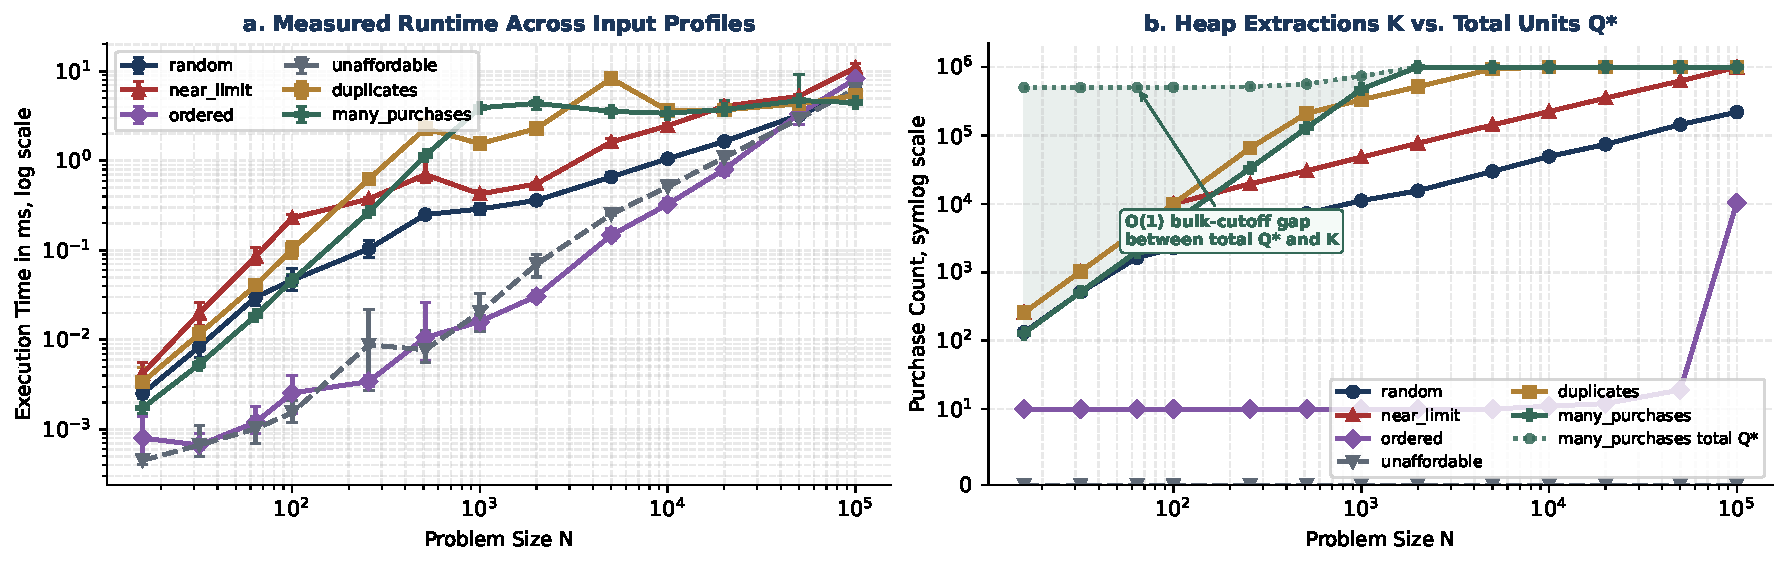
\includegraphics[width=0.98\textwidth]{runtime_and_k_scaling.pdf}
\caption{\footnotesize Solver runtime scaling and heap-extraction count $K$ versus total units $Q^*$ across problem sizes.}
\label{fig:runtime_k}
\end{figure}
\vspace{-0.35em}

\begin{figure}[H]
\centering
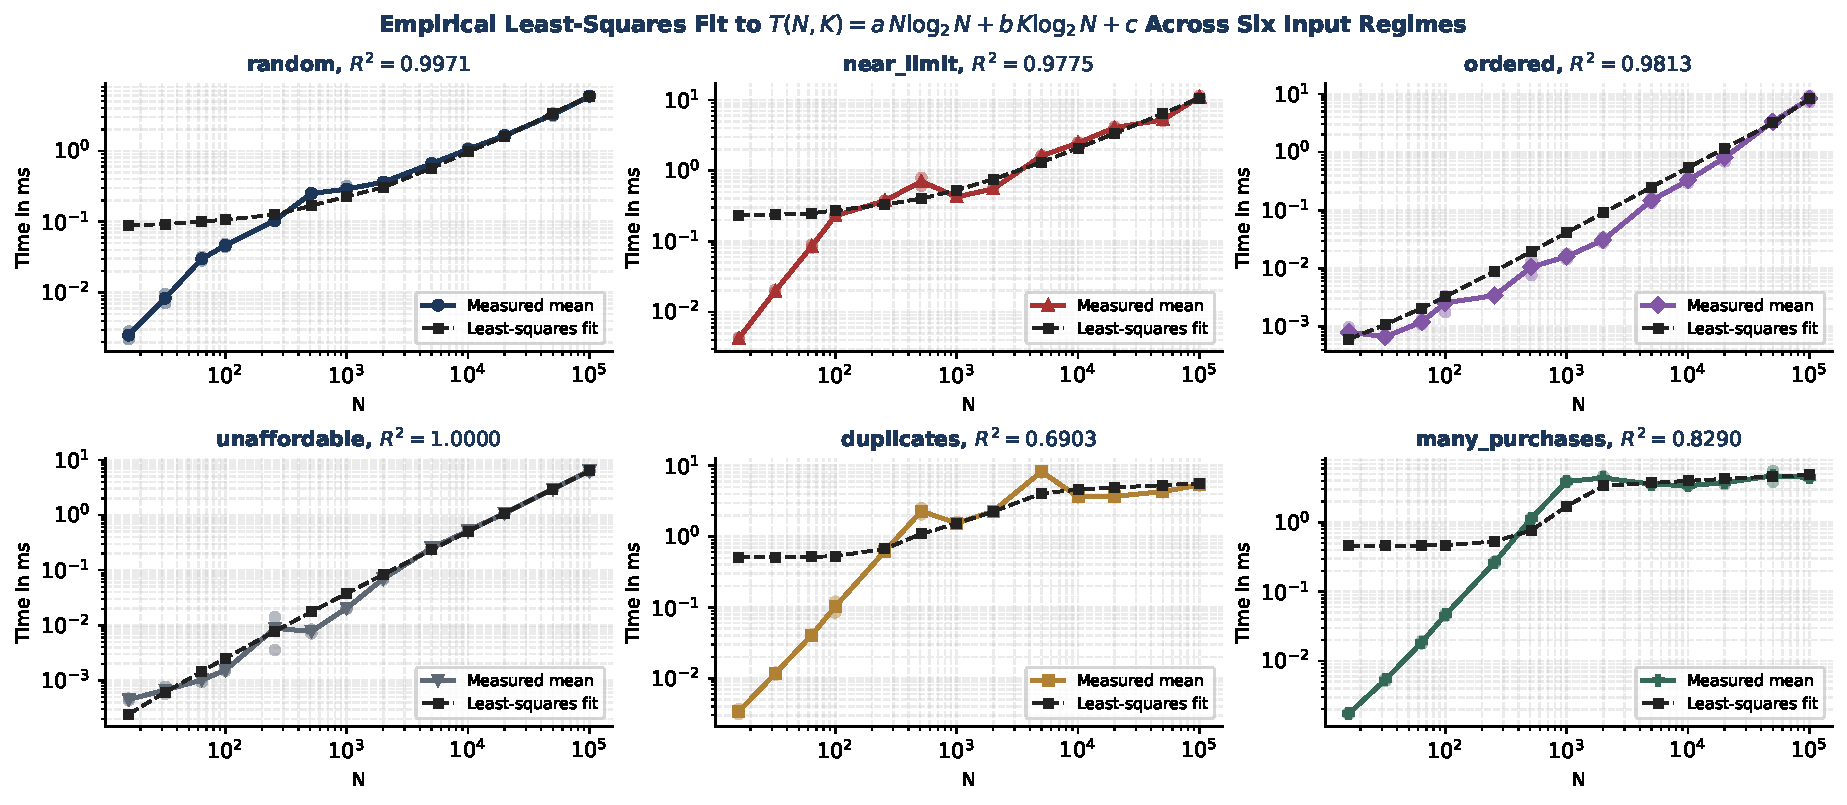
\includegraphics[width=0.98\textwidth]{complexity_fit_grid.pdf}
\caption{\footnotesize Per-profile non-negative least-squares fit to $T(N, K) = a\,N\log_2 N + b\,K\log_2 N + c$ across six input regimes.}
\label{fig:fit_grid}
\end{figure}
\vspace{-0.35em}

\begin{figure}[H]
\centering
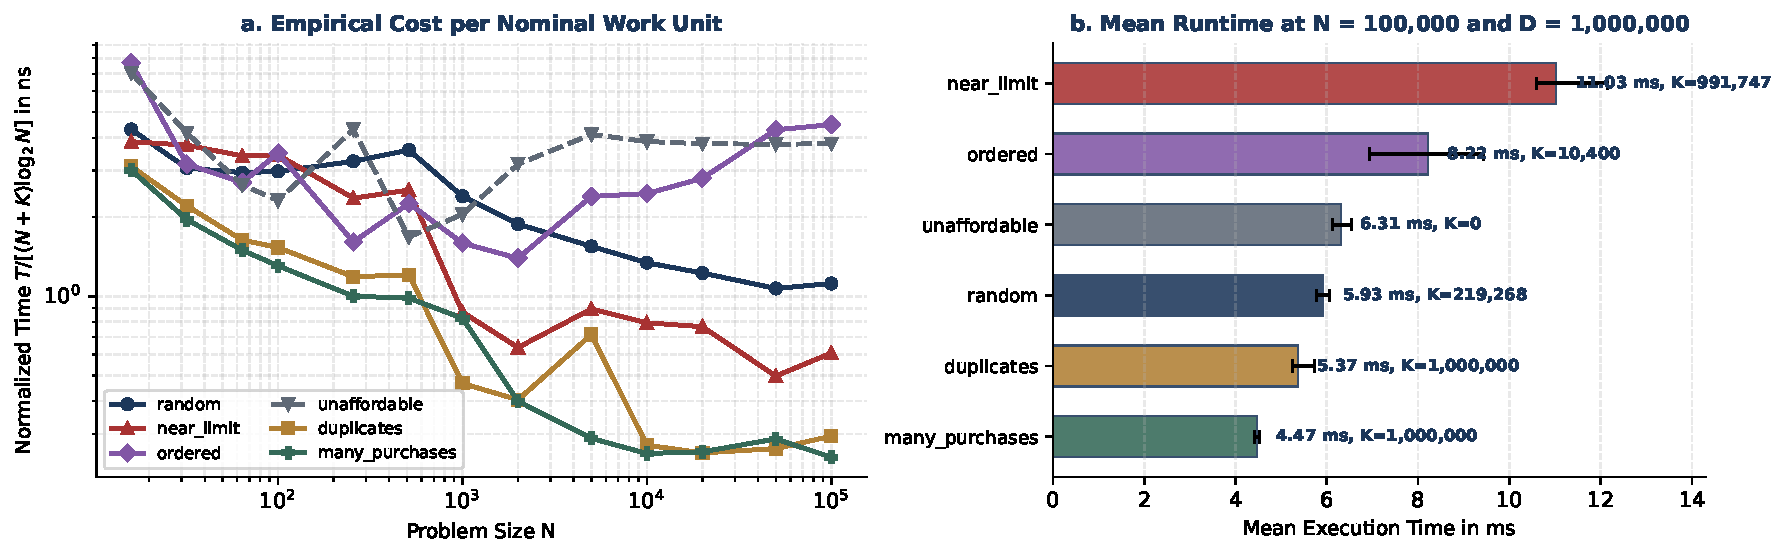
\includegraphics[width=0.98\textwidth]{normalized_work_and_regimes.pdf}
\caption{\footnotesize Normalized runtime per nominal work unit across problem sizes and cross-profile comparison at large scale.}
\label{fig:norm_regimes}
\end{figure}

\clearpage

% ============================================================
%  CHAPTER 4: ANALYSIS AND COMMENTS
% ============================================================
\section{Analysis and Comments}

\subsection{Optimality and Time/Space Complexity Analysis}
Let $N$ denote the number of item and coupon types, $D$ denote the budget, $B = \min_{1 \le i \le N} P_i$ denote the minimum full price, $M = \bigl|\{(i, j) \in \{1, \ldots, N\}^2 : P_i - C_j < B\}\bigr|$ denote the number of couponed pairs strictly cheaper than $B$, and $K = \min(Q^*, M) \le \min(N^2, D)$ denote the number of heap extractions executed by \code{solveShoppingCounted}. \Cref{tab:complexities} compares naive pair materialization, our min-heap frontier solver, and the threshold-search oracle.

\begin{table}[H]
\centering
\caption{Asymptotic time and auxiliary space comparison across exact approaches.}
\label{tab:complexities}
\setlength{\tabcolsep}{2.9pt}
\footnotesize
\begin{tabular}{@{}lcccc@{}}
\toprule
\textbf{\color{primary}Algorithm} & \textbf{\color{primary}Best Time} & \textbf{\color{primary}Avg.\ / Param.\ Time} & \textbf{\color{primary}Worst-Case Time} & \textbf{\color{primary}Space} \\
\midrule
Naive $N^2$-Pair Sort & $\Theta(N^2)$ & $\Theta(N^2 \log N)$ & $O(N^2 \log N)$ & $\Theta(N^2)$ \\
\textbf{Min-Heap}, \code{solveShopping} & $\Theta(N)$ & $O\bigl((N + K)\log N\bigr)$ & $O\bigl(N^2 + (N + K)\log N\bigr)^\dagger$ & $\Theta(N)$ \\
Threshold Search, \code{oracle} & $\Theta(N \log N + N \log D)$ & $O(N \log N + N \log D)$ & $O(N \log N + N \log D)^\ddagger$ & $\Theta(N)$ \\
\bottomrule
\multicolumn{5}{@{}p{0.96\linewidth}@{}}{\scriptsize $^\dagger$Custom median-of-three three-way \code{quickSort} has $O(N\log N)$ average time and $\Theta(N)$ time on all-equal keys, but still has $O(N^2)$ worst-case time on adversarial inputs while keeping call-stack depth at $O(\log N)$. $^\ddagger$Assuming an $O(N \log N)$ worst-case system \code{qsort}.}
\end{tabular}
\end{table}

\begin{lemmabx}{Lemma 1: Per-Item Frontier Invariant and Exactness of Bulk Cutoff}
After sorting $C_{(0)} \ge \cdots \ge C_{(N-1)}$, at the start of extraction step $r \in \{0, \ldots, K\}$, min-heap $\mathcal{H}$ contains $(P_i - C_{(\id{idx}_i)}, i)$ for every item $i$ with $\id{idx}_i < N$, where coupons $0, \ldots, \id{idx}_i - 1$ have already been popped. Hence $\id{getMin}(\mathcal{H})$ equals the minimum unredeemed discounted price across all $N^2$ pairs, and halting heap extraction once $\mathcal{H} = \emptyset$ or $\id{getMin}(\mathcal{H}) \ge B$ yields $K = \min(Q^*, M)$.
\end{lemmabx}

\begin{proof}
At $r = 0$, $\id{idx}_i = 0$ and $(P_i - C_{(0)}, i)$ is inserted into $\mathcal{H}$ for every $i$. Suppose the invariant holds before step $r + 1$. Since $C_{(0)} \ge \cdots \ge C_{(N-1)}$, every unredeemed pair $(i, j)$ has $j \ge \id{idx}_i$ and hence $P_i - C_{(\id{idx}_i)} \le P_i - C_{(j)}$, giving
\[
  \min_{\substack{0 \le i < N \\ \id{idx}_i \le j < N}} \bigl(P_i - C_{(j)}\bigr)
  \;=\; \min_{\substack{0 \le i < N \\ \id{idx}_i < N}} \bigl(P_i - C_{(\id{idx}_i)}\bigr)
  \;=\; \id{getMin}(\mathcal{H}).
\]

Popping $(P_v - C_{(\id{idx}_v)}, v)$, advancing $\id{idx}_v \gets \id{idx}_v + 1$, and inserting $(P_v - C_{(\id{idx}_v)}, v)$ when $\id{idx}_v < N$ restores the invariant. Because extracted keys are non-decreasing, the loop pops strictly all affordable pairs below $B$, stopping at $K = Q^* \le M$ if budget runs out first or at $K = M \le Q^*$ once $\mathcal{H} = \emptyset$ or $\id{getMin}(\mathcal{H}) \ge B$; thus $K = \min(Q^*, M)$.
\end{proof}

\begin{theorembx}{Theorem 1: Greedy Optimality and $O((N + K)\log N)$ Average Complexity}
Algorithm~2 returns the exact optimal pair $(Q^*, R^*)$ in Equation~\ref{eq:lex-opt}, running in $O((N + K)\log N)$ average-case time, $\Theta(N)$ best-case time, and $\Theta(N)$ auxiliary space.
\end{theorembx}

\begin{proof}
Let $U = \langle u_1 \le u_2 \le \cdots \rangle$ sort the multiset of all $N^2$ discounted prices $\{P_i - C_j\}$ together with infinitely many copies of $B = \min_i P_i$. In any feasible plan $(x, y)$ buying $q = Q(x, y)$ units with $E(x, y) \le D$, replacing full-price units of items with $P_i > B$ by item $i^* \in \arg\min_i P_i$ preserves $q$ without increasing cost, so $(x, y)$ selects $q$ elements from $U$ and obeys
\[
  E(x, y) \;\ge\; \sum_{r=1}^{q} u_r, \qquad
  Q^* \;=\; \max\Bigl\{ q \ge 0 \,\Bigm|\, \sum_{r=1}^{q} u_r \le D \Bigr\}, \qquad
  R^* \;=\; D - \sum_{r=1}^{Q^*} u_r.
\]
By Lemma~1, Algorithm~2 pops $u_1, \ldots, u_K < B$ from $\mathcal{H}$ and buys $Q^* - K = \bigl\lfloor (D - \sum_{r=1}^{K} u_r)/B \bigr\rfloor$ copies of $u_{K+1} = \cdots = u_{Q^*} = B$ in Step~6, returning $(Q^*, R^*)$.

For average-case time, three-way \code{quickSort}, $N$ initial \code{siftup} insertions, $K$ heap extractions and re-insertions, and one $O(1)$ division yield
\[
  T_{\text{avg}}(N, K) \;=\; O(N \log N) + O(N \log N) + \sum_{r=1}^{K} O(\log N) + O(1) \;=\; O\bigl((N + K)\log N\bigr),
\]
using $\Theta(N)$ auxiliary space. When all $C_j$ are equal, $P_i$ is non-decreasing, and $K = O(1)$, three-way partitioning and $O(1)$ root checks give $T_{\text{best}}(N) = \Theta(N)$.
\end{proof}

\paragraph{Byte-Level Space Accounting.}
In \code{solveShoppingCounted}, \code{items} allocates $N \times \code{sizeof(Item)} = 8N$ bytes, \code{heap->data} allocates $8N$ bytes, and \code{heap->vertices} allocates $4N$ bytes, while tail-call-eliminated \code{quickSort} uses at most $\lfloor \log_2 N \rfloor \le 16$ stack frames. At $N = 100{,}000$, heap memory totals $20N = 2{,}000{,}000$ bytes, or $\mathbf{1.91\,\text{MiB}}$---fitting entirely inside CPU L3 cache and reducing memory by over $\mathbf{20{,}000\times}$ relative to the $37.25\,\text{GiB}$ needed to store $N^2 = 10^{10}$ 4-byte pairs.

\subsection{Empirical Performance Insights Across Regimes}
Three key findings connect the theoretical bounds above to the empirical curves and least-squares fits in Chapter~3.

\vspace{-0.2em}
\begin{insightbox}{Key Finding 1: Distinct-Key Regimes Track $a\,N\log_2 N + b\,K\log_2 N + c$}
On \code{unaffordable}, every net price exceeds $4.99 \times 10^8 > D$, forcing $K = 0$ and isolating pure sorting plus $N$ initial heap insertions; the single-parameter fit $T \approx 3.793 \times 10^{-6}\,N\log_2 N\,\text{ms}$ achieves $\mathbf{R^2 = 1.0000}$ and reaches $6.31\,\text{ms}$ at $N = 10^5$. Adding active frontier pops in \code{random} with $K = 219{,}268$ in $5.93\,\text{ms}$ and \code{near\_limit} with $K = 991{,}747$ in $11.03\,\text{ms}$ maintains $\mathbf{R^2 = 0.9971}$ and $\mathbf{R^2 = 0.9775}$, while normalized cost stabilizes at $0.61$--$1.12\,\text{ns}$ per $(N + K)\log_2 N$ unit as L1/L2 cache locality amortizes sequential parallel-array accesses.
\end{insightbox}
\vspace{-0.3em}

\begin{insightbox}{Key Finding 2: Duplicate-Key Collapse Accelerates Tie-Heavy Regimes}
At $N = 100{,}000$, \code{many\_purchases} executes $K = 10^6$ heap pops in $\mathbf{4.47\,\text{ms}}$, or $0.24\,\text{ns/unit}$---faster than \code{unaffordable} at $\mathbf{6.31\,\text{ms}}$ with $K = 0$. Two concrete code paths explain both this speedup and the lower linear-log $R^2$ values of $0.8290$ and $0.6903$:
\begin{itemize}
  \item \textbf{$\Theta(N)$ Three-Way Partitioning:} In \code{many\_purchases}, $C_j \equiv 1$ places all $10^5$ coupons into the middle equality zone \code{a[lt..gt]} on the very first partition pass with zero recursive calls, whereas \code{unaffordable} sorts $10^5$ wide-range values in $C_j \in [1, 10^6]$.
  \item \textbf{$O(1)$ Early Sift Termination on Tied Roots:} In \code{duplicates} with $P_i \in [100, 105]$ and $C_j \in [95, 99]$, roughly $N^2 / 30$ pairs achieve minimum cost $100 - 99 = 1$. At $N = 5{,}000$, $N^2/30 \approx 8.33 \times 10^5 < D = 10^6$, so mixed keys $1$ and $2$ trigger deeper heap sifts taking $8.28\,\text{ms}$. Once $N \ge 10{,}000$, $N^2/30 \ge 3.33 \times 10^6 > D$: the upper $\approx N/6$ heap nodes all hold key $1$, and re-inserting key $1$ stops immediately in \code{siftup} via \code{data[index] >= data[parent]}, dropping runtime from $8.28\,\text{ms}$ at $N = 5{,}000$ to $\mathbf{3.65\,\text{ms}}$ at $N = 10{,}000$ and $\mathbf{5.37\,\text{ms}}$ at $N = 10^5$.
\end{itemize}
\end{insightbox}
\vspace{-0.3em}

\begin{insightbox}{Key Finding 3: $O(1)$ Bulk Cutoff and Affordability Threshold}
At $N = 16$ on \code{many\_purchases}, only $K = 128$ pairs satisfy $P_i - C_j = 1 < B = 2$; Step~6 then buys all remaining $Q^* - K = \mathbf{499{,}936}$ units in one integer division within $0.0017\,\text{ms}$, avoiding $99.97\%$ of the $500{,}064$ heap iterations a naive priority-queue loop would execute. Meanwhile, on \code{ordered} where $P_i = 100{,}001 + i$ and $\max C = N$, minimum discounted cost $100{,}001 - N$ stays above $50{,}001$ with $K \le 19$ for all $N \le 50{,}000$ before plunging to $1$ at $N = 100{,}000$, causing the sharp jump to $K = 10{,}400$ and $8.22\,\text{ms}$ in \Cref{fig:runtime_k}.
\end{insightbox}

\subsection{Further Possible Improvements}
Two standard enhancements from the course textbook~\cite{weiss1996} can further tighten worst-case guarantees and constant factors:
\begin{enumerate}[label=\textbf{\color{primary}\arabic*.}]
  \item \textbf{Worst-Case $O(N \log N)$ Sorting via HeapSort Fallback:} Replacing custom QuickSort with HeapSort or switching to in-place HeapSort if recursion depth exceeds $2\lfloor \log_2 N \rfloor$ guarantees deterministic $O(N \log N)$ worst-case sorting time while retaining $\Theta(N)$ duplicate handling.
  \item \textbf{Linear-Time \code{BuildHeap} and In-Place Root \code{siftdown}:} Constructing $\mathcal{H}$ bottom-up via \code{siftdown} from $\lfloor N/2 \rfloor - 1$ down to $0$ cuts initial heap construction from $O(N \log N)$ to $\Theta(N)$~\cite{weiss1996}. Moreover, when $\id{idx}_v + 1 < N$, overwriting \code{heap->data[0]} directly with $P_v - C_{(\id{idx}_v + 1)}$ and calling a single \code{siftdown(0)} avoids the intermediate leaf swap plus \code{siftup} in each purchase step.
\end{enumerate}

\clearpage

% ============================================================
%  AUTHOR LIST, DECLARATION, AND REFERENCES
% ============================================================
\section*{Author List and Declaration}
\addcontentsline{toc}{section}{Author List and Declaration}

\subsection*{Author List}
{\sloppy
\ifpeerreview
\begin{itemize}
  \item \textbf{\color{primary}Student A:} Implemented the greedy min-heap solver \code{shopping\_with\_cunpons.h}, array-backed \code{binary\_min\_heap.h}, three-way \code{quick\_sort.h}, dataset generator \code{generate.c}, oracle timing harness \code{testbench.c}, and fitting script \code{plot\_complexity.py}.
  \item \textbf{\color{primary}Student B:} Conducted benchmark verification and visualization in \code{visualization.py}, documented source files, proved greedy optimality and complexity bounds, and authored this report.
\end{itemize}
\else
\begin{itemize}
  \item \textbf{\color{primary}Yixiang Chen:} Implemented the greedy min-heap solver \code{shopping\_with\_cunpons.h}, array-backed \code{binary\_min\_heap.h}, three-way \code{quick\_sort.h}, dataset generator \code{generate.c}, oracle timing harness \code{testbench.c}, and fitting script \code{plot\_complexity.py}.
  \item \textbf{\color{primary}Runhui Lin:} Conducted benchmark verification and visualization in \code{visualization.py}, documented source files, proved greedy optimality and complexity bounds, and authored this report.
\end{itemize}
\fi
}

\subsection*{Declaration}
We hereby declare that all the work done in this project titled ``Shopping with Coupons: Greedy Min-Heap Selection and Analysis'' is of our independent effort as a group.

\subsection*{Signatures}
\vspace{0.35cm}
\noindent
\ifpeerreview
\begin{minipage}[t]{0.48\linewidth}
\centering
\vspace{1.15cm}
\rule{0.92\linewidth}{0.4pt}\\[0.15cm]
Student A
\end{minipage}\hfill
\begin{minipage}[t]{0.48\linewidth}
\centering
\vspace{1.15cm}
\rule{0.92\linewidth}{0.4pt}\\[0.15cm]
Student B
\end{minipage}
\else
\begin{minipage}[t]{0.48\linewidth}
\centering

\includegraphics[height=1.35cm,keepaspectratio]{signature_chen.png}\\[-0.1cm]
\rule{0.92\linewidth}{0.4pt}\\[0.15cm]
Yixiang Chen
\end{minipage}\hfill
\begin{minipage}[t]{0.48\linewidth}
\centering

\includegraphics[height=1.55cm,keepaspectratio]{signature_lin.png}\\[-0.1cm]
\rule{0.92\linewidth}{0.4pt}\\[0.15cm]
Runhui Lin
\end{minipage}
\fi

\vspace{0.6cm}
\printbibliography[heading=bibintoc]

\clearpage

% ============================================================
%  APPENDIX
% ============================================================
\appendix
\titleformat{\section}
  {\color{primary}\centering\Large\bfseries}
  {\color{accent}Appendix~\thesection.}{0.6em}{}
  [\vspace{0.3em}{\color{accent!70}\titlerule[1.5pt]}]

\section{Source Code}

All source files reside in \code{src/} with strictly over $30\%$ commented lines in every C11 header and source file. Below we list the solver interface, three-way QuickSort, parallel-array binary min-heap, greedy frontier solver with bulk cutoff, interactive CLI demo, cross-platform path helper, dataset generator, verification/timing harness, and Python complexity/visualization scripts.

\subsection{Solver Result Interface: \texttt{bench.h}}
\lstinputlisting[language=C]{../src/bench.h}

\subsection{Descending Three-Way QuickSort: \texttt{quick\_sort.h}}
\lstinputlisting[language=C]{../src/quick_sort.h}

\subsection{Parallel-Array Binary Min-Heap: \texttt{binary\_min\_heap.h}}
\lstinputlisting[language=C]{../src/binary_min_heap.h}

\subsection{Greedy Frontier Solver with Bulk Cutoff: \texttt{shopping\_with\_cunpons.h}}
\lstinputlisting[language=C]{../src/shopping_with_cunpons.h}

\subsection{Interactive Standard-Input Demo Driver: \texttt{testbench\_demo.c}}
\lstinputlisting[language=C]{../src/testbench_demo.c}

\subsection{Cross-Platform Project Root Resolver: \texttt{project\_paths.h}}
\lstinputlisting[language=C]{../src/project_paths.h}

\subsection{Deterministic 158-Case Dataset Generator: \texttt{generate.c}}
\lstinputlisting[language=C]{../src/generate.c}

\subsection{Threshold-Oracle Verification and Timing Harness: \texttt{testbench.c}}
\lstinputlisting[language=C]{../src/testbench.c}

\subsection{Non-Negative Least-Squares Regression Script: \texttt{plot\_complexity.py}}
\lstinputlisting[language=Python]{../src/plot_complexity.py}

\subsection{Report Vector Visualization Script: \texttt{visualization.py}}
\lstinputlisting[language=Python]{../src/visualization.py}

\end{document}
